\documentclass{beamer}[10]
\usepackage{pgf}
\usepackage[danish]{babel}
\usepackage[utf8]{inputenc}
\usepackage{beamerthemesplit}
\usepackage{graphics,epsfig, subfigure}
\usepackage{url}
\usepackage{srcltx}
\usepackage{hyperref}
\usepackage{ragged2e}
\usepackage{cancel} % para poder colocar o tracinho de cancelamento


\graphicspath{{./images/}} % set an default images folder

\definecolor{kugreen}{RGB}{50,93,61}
\definecolor{kugreenlys}{RGB}{132,158,139}
\definecolor{kugreenlyslys}{RGB}{173,190,177}
\definecolor{kugreenlyslyslys}{RGB}{214,223,216}
\setbeamercovered{transparent}
\mode<presentation>
\usetheme[numbers,totalnumber,compress,sidebarshades]{PaloAlto}
\setbeamertemplate{footline}[frame number]
\justifying

  \usecolortheme[named=kugreen]{structure}
  \useinnertheme{circles}
  \usefonttheme[onlymath]{serif}
  \setbeamercovered{transparent}
  \setbeamertemplate{blocks}[rounded][shadow=true]

\logo{
\includegraphics[width=1.55cm]{img00_UEA.png}}
%\useoutertheme{infolines} 

\title[Micro II]{Microeconomia II - 2021/02}
\author{Bruno de M. Ruas} 
\institute{Escola Superior de Ciências Sociais\\Universidade do Estado do Amazonas}
\date{\today}

\begin{document}

% pagina de titulo
\frame{\titlepage \vspace{-0.5cm}} 

% Sumario
\frame{
\frametitle{Sumário}
\tableofcontents
}

%%%%%%%%%%%%%%%%%%%%%%%%%%%%%%%%%%%%%%%%%%%
\section{Introdução}
%%%%%%%%%%%%%%%%%%%%%%%%%%%%%%%%%%%%%%%%%%%

\begin{frame}
	\Huge Introdução
\end{frame}

\begin{frame}
	\frametitle{Apresentação do Professor}
	Nome: Bruno de Melo Ruas
	\\~\\
	Formação:
	\begin{itemize}
		\item Graduação em Ciências Econômicas (UEA) em 2017
		\item Pós-graduação em Gestão Financeira (FGV) em 2020
		\item Cursando Análise e Desenvolvimento de Sistemas (PUC-MG)
	\end{itemize}

	Experiência:
	\begin{itemize}
		\item Monitorias de Intro. Eco, Macro I e Econometria
		\item Projeto Acadêmico de Iniciação Científica
		\item Observatório do Polo Industrial (UEA)
		\item Gerente de Orçamento da SEMSA-Manaus (2019-2020)
		\item Supervisor de Faturamento One Clinic (Atualmente)
	\end{itemize}
\end{frame}

\begin{frame}
	\frametitle{Ementa do Curso}
	\begin{itemize}
		\item Poder de Mercado;
		\item Monopólios e Monopsônios;
		\item Mercado de Fatores;
		\item Interação estratégica;
		\item Oligopólios: Equilíbrios de Cournot e Bertrand;
		\item Introdução à Teoria dos Jogos: Estratégias dominantes, Equilíbrio de Nash;
		\item Jogos dinâmicos, Jogos sequenciais;
		\item Introdução ao equilíbrio geral;
		\item Falhas de Mercados e ineficiência do equilíbrio;
		\item Externalidades;
		\item Bens Públicos;
		\item Assimetria de Informação.
	\end{itemize}
\end{frame}

\begin{frame}
	\frametitle{Bibliografia}
	\begin{itemize}
		\item Varian, Hal. Microeconomia: Uma Abordagem Moderna. 6 ed. Rio de Janeiro: Campus Elsevier, 2003. (Principal)
		\item Goolsbee, Levitt e Syverson. Microeconomia. 2 ed. São Paulo: Atlas, 2008.
		\item Pindyck, Robert S.; Rubinfeld, Daniel L. Microeconomia. 6 ed. São Paulo: Pearson Prentice Hall, 2007.
		\item Bergstrom, Theodore C.; Varian, Hal R. Workouts in intermediate microeconomics. WW Norton, 2014.
		\item Varian, Hal R. Intermediate microeconomics with calculus: a modern approach. WW Norton \& Company, 2014.
	\end{itemize}
\end{frame}

\begin{frame}
	\frametitle{Metodologia}
	
	Professor:
	\begin{itemize}
		\item Aulas expositivas e dinâmicas (EAD ou presenciais) com os conteúdos propostos
		\item Material didático original elaborado específicamente para o curso (versão 1.0)
		\item Grupo no discord para tiragem de dúvidas e auxílios extra-classe
		\item Publicação de todo o material no repositório do Github
	\end{itemize}

	Alunos:
	\begin{itemize}
		\item Presença participativa em todas as aulas e, em caso de falta, esforço de recuperação do material perdido
		\item Leitura antecipada do material referente à cada aula prevista
		\item Realização dos exercícios propostos em sala de aula e para casa
	\end{itemize}

\end{frame}

\begin{frame}
	\frametitle{Panorama do Curso}

	Como o nome da disciplina deixa evidente, nós estamos continuando uma jornada que já se iniciou com a disciplina de Microeconomia I.
	\\~\\
	A essa altura, você deve ter o domínio de assuntos como:
	\begin{itemize}
		\item O Modelo de Escolha do Consumidor
		\begin{itemize}
			\item Restrição Orçamentária
			\item Curvas de Indiferença
			\item Excedente do Consumidor
		\end{itemize}
		\item A Oferta da Empresa competitiva
		\begin{itemize}
			\item Custos: Médio, Marginal, Total
			\item Curvas de isolucro
			\item Tecnologias de Produção 
		\end{itemize}
		\item Mercado de Fatores
		\item O Equilíbrio de Mercado competitivo
	\end{itemize}
\end{frame}

\begin{frame}
	\frametitle{Panorama do Curso}
	Os ferramentais usados ao longo do curso de microeconomia I também não devem ser nenhum mistério. Portanto, vocês já devem saber o que são:
	\\~\\
	\begin{itemize}
		\item Funções, funções Inversas, funções lineares, coeficientes angular e linear
		\item Variações e Taxas de Variação
		\item Derivadas e Derivadas Parciais
		\item Otimização e Otimização com Restrição
	\end{itemize}
	Então podemos seguir de onde micro I parou, né?
\end{frame}

\begin{frame}
	\frametitle{Panorama do Curso}
	\begin{center}
		
\includegraphics[scale=0.4]{img01.jpg}
	\end{center}
\end{frame}

%%%%%%%%%%%%%%%%%%%%%%%%%%%%%%%%%%%%%%%%%%%
\section{Preparativos}
%%%%%%%%%%%%%%%%%%%%%%%%%%%%%%%%%%%%%%%%%%%

\begin{frame}
	\Huge Preparativos
\end{frame}

\begin{frame}
	\frametitle{Funções}
	Vamos relembrar as principais ferramentas  matemáticas necessárias para compreender alguns livros de microeconomia de graduação.
	\begin{block}{Funções}
		Sejam dois números quaisquer $x$ e $y$, uma \textbf{função} ou \textbf{transformação} é uma regra que descreve uma relação entre eles.
	\end{block}

	\begin{block}{Propriedades das Funções}
		Uma \textbf{função contínua} é aquela que não possui nenhum "salto"\ ou "quebra".\\
		Uma \textbf{função suave} é aquela que não tem "dobras"\ nem "cantos".\\
		Uma \textbf{função monotônica} é aquela que sempre segue o mesmo sentido (ou crescendo ou decrescendo) sem nunca mudar de sentido.
	\end{block}
\end{frame}

\begin{frame}
	\frametitle{Funções}

	Essas definições são simplificações draconianas dos conceitos que os matemáticos desenvolveram. Como o escopo do curso é introdutório, precisaremos nos valer dessas versões mais simples.
	\\~\\
	Quando é uma função é crescente a medida que $x$ cresce, chamaremos de \textbf{função monotônica crescente}. Quando decrescer a medida que $x$ crescer, chamaremos de \textbf{função monotônica decrescente}.

	\begin{block}{Função Inversa}
		Uma \textbf{função inversa} é a função que, sempre que colocarmos um $y$ como variável independente teremos como resultado um $x$ de alguma função anterior.
	\end{block}
\end{frame}

\begin{frame}
	\frametitle{Funções}

	\begin{block}{Função Linear}
		Chamamos de \textbf{função linear}, qualquer função da forma $y = ax + b$.
	\end{block}
	Fique atento porque uma função linear pode ser expressa de maneira implícita (ou seja, será necessário desenvolver um pouco a álgebra até que se chegue numa equação no formato da definição).
\end{frame}

\begin{frame}
	\frametitle{Equações e Identidades}
		
	\begin{block}{Equações}
		\textbf{equações} (usando o símbolo da igualdade "$=$"). Onde as suas respectivas \textbf{soluções} são os valores atribuíveis as incógnitas que assegurem a validade da relação proposta.
	\end{block}

	\begin{block}{Identidades}
		Uma \textbf{identidade} (que tem o símbolo dado por "$\equiv$") é um tipo de relação onde sempre haverá as soluções independentemente de quais valores suas variáveis assumam.
	\end{block}
\end{frame}

\begin{frame}
	\frametitle{Variações}

	\begin{block}{Variações}
		Usamos o símbolo "$\Delta$"\footnote{O nome é "delta".} para denotar a variação de alguma variável. Ou seja, se tivemos uma variável qualquer $x$ que teve seu valor alterado de $x^1$ para $x^2$, então:
		$$ \Delta x = x^2 - x^1 $$
		ou também
		$$ x^2 = x^1 + \Delta x $$
	\end{block}

	Normalmente, usamos o delta quando falamos de \textbf{pequenas variações} ou, como os economistas falam, \textbf{variações marginais}.
\end{frame}

\begin{frame}
	\frametitle{Taxa de Variação}

	\begin{block}{Taxa de Variação}
		A \textbf{taxa de variação} é obtida pela razão (ou seja, pela divisão) de duas variações. Seja a função $y = f(x)$, sempre que tivermos um $\Delta x > 0$ e também tivermos algum $\Delta y \neq 0$. A taxa de variação de $y$ em relação à $x$ é dada por:
		$$ \frac{\Delta y}{\Delta x} = \frac{y^2 - y^1}{x^2 - x^1} = \frac{f(x^1 + \Delta x) - f(x^1)}{\Delta x} $$
	\end{block}

	É uma medida do quanto $y$ varia a medida que $x$ varia.
\end{frame}

\begin{frame}
	\frametitle{Taxa de Variação}
	Quando uma função é linear, teremos que essa taxa de variação será sempre constante para quaisquer valores de $x$. Como $y = ax + b$, então
	\\~\\
	\Large $ \frac{\Delta y}{\Delta x} = $ \small
	$$ \frac{a(x^1 + \Delta x) + b - (ax^1 + b)}{\Delta x} = $$
	$$ \frac{ax^1 + a\Delta x + b - ax^1 - b}{\Delta x} = $$
	$$ \frac{ax^1 + a\Delta x \cancel{+ b} - ax^1 \cancel{- b}}{\Delta x} = $$
	$$ \frac{ax^1 + a\Delta x - ax^1}{\Delta x} = $$
	$$ \frac{\cancel{ax^1} + a\Delta x \cancel{- ax^1}}{\Delta x} = \frac{a \cancel{\Delta x}}{\cancel{\Delta x}} = a $$
\end{frame}

\begin{frame}
	\frametitle{Taxa de Variação}

	Para as funções não lineares, essa propriedade não é observada. Tomemos $y = f(x) = x^2$ como exemplo,
	\\~\\
	\Large $ \frac{\Delta y}{\Delta x} = $ \normalsize
	$$ \frac{(x + \Delta x)^2 - x^2}{\Delta x} = $$ 
	$$  \frac{\cancel{x^2} + 2x \Delta x + (\Delta x)^2 \cancel{-x^2}}{\Delta x} = $$
	$$  \frac{2x \cancel{\Delta x} + \Delta x . \cancel{\Delta x}}{\cancel{\Delta x}} = $$
	$$  2x + \Delta x $$
\end{frame}

\begin{frame}
	\frametitle{Inclinações e Interceptos}
	
	\begin{block}{Inclinações}
		Em uma função linear, a inclinação da curva sempre será a mesma independente da magnitude da variação.\\
		No caso das funções não lineares, a inclinação é dada pela \textbf{reta tangente} ao ponto da curva.
	\end{block}

	\begin{block}{Interceptos}
		No caso de uma função linear, $ y = ax + b$, temos alguns pontos que recebem nomes de \textbf{intercepto}. O \textbf{intercepto vertical} ($y^*$) é dado pelo ponto $y = a.0 + b = b$, ou seja, onde $x = 0$. Já o \textbf{intercepto horizontal} ($x^*$) é dado pelo ponto onde $y = ax + b = 0 $, ou seja, $ x = \frac{-b}{a}$
	\end{block}
\end{frame}

\begin{frame}
	\frametitle{Valor Absoluto e Logaritmo}

	\begin{block}{Valor Absluto}
		O \textbf{valor absoluto} de um número $x$ qualquer é definido pela função $f(x)$ do seguinte modo:

		\[ f(x) = |x| = \begin{cases} x & se \ x \geqslant \\ -x & se \ x < 0 \end{cases} \]
	\end{block}

	\begin{block}{Logaritmo Natural}
		Você já deve ter visto no ensino médio que o \textbf{logaritmo natural} ou \textbf{log} de um número é uma função escrita como $y = lnx$ ou $y = ln(x)$ e que possui as seguintes propriedades:

		\begin{itemize}
			\item Se $x,y > 0$, então, $ ln(xy) = ln(x) + ln(y) $
			\item $ ln(e) = 1 $
			\item $ ln(x^y) = y ln(x) $
		\end{itemize}
	\end{block}
\end{frame}

\begin{frame}
	\frametitle{Derivadas}

	Você deve lembrar desse conceito das aulas de matemática no primeiro período.
	\\~\\
	\begin{block}{Derivada}
		A \textbf{derivada} da função $f(x)$ será dada por:

		$$ f'(x) = \frac{df(x)}{dx} = \lim_{\Delta x \to 0} \frac{f(x + \Delta x) - f(x)}{\Delta x} $$
	\end{block}
	A gente acabou de ver um conceito muito parecido na parte de Taxa de Variação. E é isso mesmo, a derivada é o cálculo da taxa de variação à medida que aplicamos o limite tendendo a zero na variação de $(\Delta x)$.
\end{frame}

\begin{frame}
	\frametitle{Derivadas}

	\textbf{Comentário}: Essa técnica é muito importante ao longo de quase todos os tópicos desse curso. Volte nas apostilas e nas listas de derivadas caso seja necessário.
	\\~\\
	Já vimos que a deriva nos permite saber a inclinação da reta tangente da nossa função genérica $f(x)$ num determinado ponto.
	
	\begin{block}{Derivadas Segundas}
		Chamamos de \textbf{derivada segunda} de $f(x)$ a derivada da derivada dessa função.

		$$ f''(x) = \frac{d^2f(x)}{dx^2} $$
	\end{block}

	Se for positiva, a função é convexa no ponto. Se for negativa, a função é côncava no ponto. Por fim, se for igual a zero, a função será plana.
\end{frame}

\begin{frame}
	\frametitle{Regra do Produto e da Cadeia}

	Dadas duas funções $g(x)$ e $h(x)$.

	\begin{block}{Regra do Produto}
		Definindo uma nova função $f(x) = g(x) h(x)$. A derivada dessa última função é dada pela aplicação da \textbf{regra do produto}:
		$$ \frac{df(x)}{dx} = g(x)\frac{dh(x)}{dx} + h(x)\frac{dg(x)}{dx}$$
	\end{block}

	Dadas as funções $y = g(x)$ e $z = h(y)$.

	\begin{block}{Regra da Cadeia}
		A \textbf{função composta} é dada por $f(x) = h(g(x))$ cuja derivada de uma função composta é obtida pela \textbf{regra da cadeia} da seguinte forma:
		$$ \frac{df(x)}{dx} = \frac{dh(y)}{dy}\frac{dg(x)}{x}$$
	\end{block}
\end{frame}

\begin{frame}
	\frametitle{Derivadas Parciais}

	Supondo uma função composta $f(x_1,x_2)$.

	\begin{block}{Derivada Parcial}
		A \textbf{derivada parcial} de $f(x_1,x_2)$ em relação a $x_1$ é  dada por:

		$$ \frac{\partial f(x_1,x_2)}{\partial x_1} = 
		\lim_{\Delta x_1 \to 0} \frac{f(x_1+\Delta x_1,x_2) - f(x_1,x_2)}{\Delta x_1} $$
		\\
		Similarmente, a derivada parcial em relação a $x_2$ será dada por:
		\\
		$$ \frac{\partial f(x_1,x_2)}{\partial x_2} = 
		\lim_{\Delta x_2 \to 0} \frac{f(x_1,x_2+\Delta x_2) - f(x_1,x_2)}{\Delta x_2} $$
	\end{block}
\end{frame}

\begin{frame}
	\frametitle{Regra da cadeia das Derivadas Parciais}

	Seja a função composta $g(t) = f(x_1(t),x_2(t))$.

	\begin{block}{Regra da Cadeia para Funções Compostas}
		A \textbf{regra da cadeia} aplicada à essa função é dada por:
		$$ \frac{dg(t)}{dt} = 
		\frac{\partial f(x_1,x_2)}{\partial x_1}\frac{dx_1(t)}{dt} + 
		\frac{\partial f(x_1,x_2)}{\partial x_2}\frac{dx_2(t)}{dt} $$
	\end{block}

	Atente para o fato que as variáveis independentes da nossa função $g(t)$ são as funções $x_1(t)$ e $x_2(t)$ que também têm como variável independente $t$.
\end{frame}

\begin{frame}
	\frametitle{Otimização}

	Matematicamente falando, dada uma função $y = f(x)$ seu valor \textbf{máximo} será dado no ponto $x^*$ se $f(x^*) \geqslant f(x)$ para qualquer valor de $x$.
	\begin{block}{Condições de Maximização}
		Se uma função for suave, o seu valor máximo é obtido no ponto onde teremos:
		$$\textrm{Condição de 1º Ordem: } \frac{df(x^*)}{dx} = 0 $$
		e também
		$$\textrm{Condição de 2º Ordem: } \frac{d^2f(x^*)}{dx^2} \leq 0$$	
	\end{block}
\end{frame}

\begin{frame}
	\frametitle{Otimização}

	Também é muito comum buscarmos a minimização de determinadas funções. Nesse caso, só teremos uma pequena mudança na condição de segunda ordem

	\begin{block}{Condições de Minimização}
		Se uma função for suave, o seu valor mínimo é obtido no ponto onde teremos:
		$$\textrm{Condição de 1º Ordem: } \frac{df(x^*)}{dx} = 0 $$
		e também
		$$\textrm{Condição de 2º Ordem: } \frac{d^2f(x^*)}{dx^2} \geq 0$$	
	\end{block}
\end{frame}

\begin{frame}
	\frametitle{Otimização}

	No casos das funções compostas suaves, as condições de primeira ordem para os pontos de máximo e mínimo são alcançadas no ponto $(x_{1}^*,x_{2}^*)$ cujas derivadas serão

	\begin{block}{Otimização de Função Composta}
		$$ \frac{\partial f(x_{1}^*,x_{2}^*)}{\partial x_1} = 0 $$
		e
		$$ \frac{\partial f(x_{1}^*,x_{2}^*)}{\partial x_2} = 0 $$
	\end{block}

	As condições de segunda ordem são muito mais complexas então não fazem parte do escopo desse curso.
\end{frame}

\begin{frame}
	\frametitle{Otimização com Restrição}

	Saber maximizar ou minimizar uma função é só uma parte do problema de otimização. Na vida real, a esmagadora maioria das situações de otimização está contida dentro de algum limite de possibilidades.
	\\~\\
	A \textbf{otimização com restrição} é a técnica usada para encontrar o ponto de máximo ou mínimo de alguma função dentro de um determinado domínio de possibilidades.

	\begin{block}{Otimização com Restrição}
		$$ \huge \stackrel{max}{\textrm{\tiny $x_1,x_2$}} \normalsize f(x_1,x_2) $$
		\normalsize $$ \textrm{de modo que } g(x_1,x_2) = c $$
	\end{block}

	A função $f(x_1,x_2)$ é chamada de \textbf{função objeto} e a equação $g(x_1,x_2) = c$ é chamada de \textbf{restrição}.
\end{frame}

\begin{frame}
	\frametitle{Otimização com Restrição}

	Quando temos uma função de uma única variável, basta transformarmos a nossa restrição em uma igualdade, substituir uma função dentro da outra e aplicar as condições de primeira e segunda ordem.

	\begin{block}{Exemplo: O Problema da Empresa Líder (cap 28.2)}
		$$ \huge \stackrel{max}{\textrm{\tiny $y_1$}} \normalsize p(y_1 + y_2)y_1 - c_1(y_1) $$
		\normalsize $$ \textrm{de modo que } y_2 = f_2(y_1) $$
	\end{block}
\end{frame}

\begin{frame}
	\frametitle{Otimização com Restrição}

	Quanto temos uma função de múltiplas variáveis, temos que lidar com tangências em ordem mais elevadas. Quando dizemos que duas curvas são tangentes, podemos afirmar que o \textbf{vetor gradiente} dessas duas curvas são proporcionais em alguma medida.
	\\~\\
	Para não dificultar, um vetor gradiente é um vetor que contém as derivadas parciais de uma função multivariada. E, como qualquer vetor, poder ser somado para indicar uma única direção.
\end{frame}

\begin{frame}
	\frametitle{Otimização com Restrição}

	Num ponto qualquer $(x_1,x_2)$ o vetor gradiente aponta para a direção onde os valores da função $f(x_1,x_2)$ aumentam mais rapidamente.
	\\~\\
	Uma propriedade interessante dos vetores gradientes é que quando duas funções são tangentes, seus vetores gradientes são proporcionais. O multiplicador de Langrange é justamente a quantidade dessa proporção.
	\\~\\
	\begin{block}{Indicação de Material}
		Esse vídeo explica muito bem como o processo de otimização com restrição faz uso do vetor gradiente.
		\\
		\begin{center}
			\href{https://www.youtube.com/watch?v=yuqB-d5MjZA}{[Clique Aqui]} 
			e
			\href{https://www.youtube.com/watch?v=hQ4UNu1P2kw}{[Clique Aqui]}
		\end{center}
	\end{block}
\end{frame}

%%%%%%%%%%%%%%%%%%%%%%%%%%%%%%%%%%%%%%%%%%%
\section{Monopólio}
%%%%%%%%%%%%%%%%%%%%%%%%%%%%%%%%%%%%%%%%%%%

\begin{frame}
	\Huge Monopólio \normalsize
	\\~\\
	\begin{itemize}
		\item Maximização dos Lucros
		\item Curva de Demanda Linear e Monopólio
		\item Estabelecimento de Preços com Markup
		\item A Ineficiência do Monopólio
		\item O Ônus do Monopólio
		\item O Monopólio Natural
		\item O que Causa os Monopólios
	\end{itemize}
\end{frame}

%%%%%%%%%%%%%%%%%%%%%%%%%%%%%%%%%%%%%%%%%%%

\begin{frame}
	\frametitle{Introdução}

	Vamos trabalhar um caso diferente do que foi visto no curso de microeconomia I: \textbf{Como seria o caso onde só exista uma empresa controlando toda a oferta?}
	\\~\\
	Diferente dos casos anteriores, agora nós buscamos construir um modelo de tomada de decisão que leve em consideração a capacidade do monopolista de intervir diretamente no preço de modo a maximizar seus lucros totais.
	\\~\\
	Existem duas maneiras de enxergar esse problema:
	\begin{itemize}
		\item Podemos modelar como se o monopolista controlasse o preço e a demanda é quem definiria a quantidade de equilíbrio.
		\item Podemos modelar como se o monopolista definisse a quantidade e a demanda definiria o seu preço de equilíbrio.
	\end{itemize}
\end{frame}

%%%%%%%%%%%%%%%%%%%%%%%%%%%%%%%%%%%%%%%%%%%

\begin{frame}
	\frametitle{Maximização dos Lucros}

	Podemos resumir o problema do monopolista como:

	\begin{block}{O problema do Monopolista}
		\LARGE $$ \stackrel{max}{\text{\small $y$}} \ \ \stackrel{r(y) - c(y)}{\ } $$
	\end{block}

	Onde $p(y)$ é a demanda inversa para o mercado, $r(y) = yp(y)$ é a receita do monopolista e $c(y)$ é o custo de produção das $y$ unidades.
\end{frame}

\begin{frame}
	\frametitle{Maximização dos Lucros}

	A condição de otimização é evidente: A receita marginal deve ser igual ao custo marginal.
	\\~\\
	Se a receita marginal for maior, bastaria aumentar a produção para aumentar os lucros. Se fosse menor, seria necessário reduzir a quantidade produzida afim de elevar o preço a um nível satisfatório.
	\\~\\
	Algebricamente, o problema é
	$$ \textrm{RM = CMa} $$
	$$ ou $$
	$$ \frac{\Delta r}{\Delta y} = \frac{\Delta c}{\Delta y} $$
\end{frame}

\begin{frame}
	\frametitle{Maximização dos Lucros}

	O custo marginal é definido pela tecnologia de produção. A mudança em relação ao modelo competitivo acontecerá na receita marginal.
	\\~\\
	Como o monopolista tem o poder de intervir no mercado, sempre que ele decidir alterar a produção em $\Delta y$ unidades, haverá dois efeitos na receita:
	\begin{itemize}
		\item Ele terá um aumento na receita em $p\Delta y$ unidades
		\item Como o mercado terá mais bens a sua disposição, ele estará disposto a pagar um preço menor pelas novas unidades, ou seja, $y\Delta p$
	\end{itemize}

	O resultado será obtido por
	$$\Delta r = p \Delta y + y \Delta p$$
\end{frame}

\begin{frame}
	\frametitle{Maximização dos Lucros}

	\small $$\Delta r = p \Delta y + y \Delta p$$

	$$ \frac{\Delta r}{\Delta y} = 
	\frac{p \Delta y}{\Delta y} + 
	\frac{y \Delta p}{\Delta y} $$

	$$ \phantom{\frac{\Delta r}{\Delta y}} = 
	\frac{p \cancel{\Delta y}}{\cancel{\Delta y}} + 
	\frac{y \Delta p}{\Delta y} $$

	$$ \phantom{\frac{\Delta r}{\Delta y}} = p + y\frac{\Delta p}{\Delta y} $$

	$$ \phantom{\frac{\Delta r}{\Delta y}} = 
	p \left[ 1 + \underbrace{\frac{y}{p}\frac{\Delta p}{\Delta y}}_\text{1/elasticidade} \right] $$

	$$ \phantom{\frac{\Delta r}{\Delta y}} = 
	p \left[ 1 + \frac{1}{\epsilon(y)} \right] $$
\end{frame}

\begin{frame}
	\frametitle{Maximização dos Lucros}

	Como a elasticidade da demanda é negativa, podemos reescrever como

	$$ \frac{\Delta r}{\Delta y} = 
	RM(y) =
	p \left[ 1 - \frac{1}{|\epsilon(y)|} \right] $$

	Veja só como sofisticamos um pouco mais a ideia da receita marginal. Agora é uma função do preço e da elasticidade-preço da demanda.
	\\~\\
	Voltemos para a condição de maximização onde a Receita Marginal deve ser igual a o Custo Marginal.

	$$ p(y) \left[ 1 - \frac{1}{|\epsilon(y)|} \right] = CMa(y) $$
\end{frame}

\begin{frame}
	\frametitle{Maximização dos Lucros}

	Não faz sentido para ele operar nos pontos onde a demanda é inelástica porque ele poderia simplesmente reduzir a quantidade produzida (o que reduziria o custo total) com aumento de receita (porque o preço aumentaria). O ponto de máximo estará sempre na zona onde $|\epsilon| \geq 1$.
	\\~\\
	Se operar no ponto onde $\epsilon$ tende ao infinito, cairá exatamente no caso da competição perfeita. Onde a receita marginal é igual ao preço.
	\\~\\
	Agora podemos ver claramente que o nosso monopolista atuará somente nos pontos onde a demanda é elástica ($|\epsilon| > 1$).

	\begin{block}{Para discussão em aula}
		O que acontece quando $|\epsilon| = 1$?
	\end{block}
\end{frame}

%%%%%%%%%%%%%%%%%%%%%%%%%%%%%%%%%%%%%%%%%%%

\begin{frame}
	\frametitle{Curva de Demanda Linear e Monopólio}
	Veremos como fica o comportamento dessas variáveis num exemplo cuja curva de demanda é linear.
	\\~\\
	Considere os seguintes sistemas de equações:
	\begin{block}{Varian pg 632}
		$$ \textrm{Demanda Linear Inversa: } p(y) = a - by $$
		$$ \textrm{Função Receita: } r(y) = p(y)y = ay - by^2 $$
		$$ \textrm{Função Receita Marginal: } RM(y) = a - 2by $$
	\end{block}

	A receita marginal é dada (capítulo 15) pela derivada da função receita. Podemos ver que o intercepto vertical da demanda e da receita marginal são iguais (dado pelo ponto $a$).
\end{frame}

\begin{frame}
	\frametitle{Curva de Demanda Linear e Monopólio}

	\begin{center}
		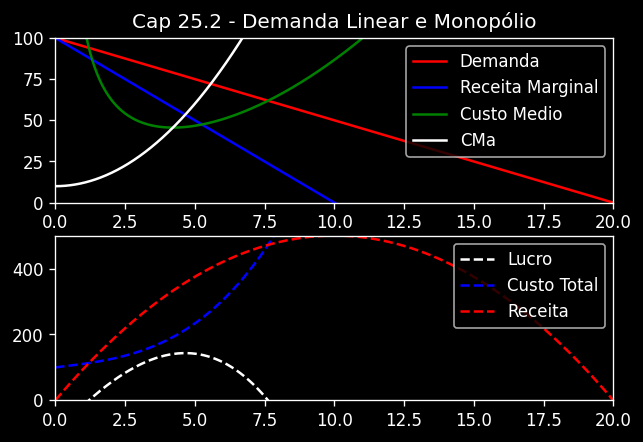
\includegraphics[scale=0.7]{cap25_2-demanda_linear_e_monopolio.png}
	\end{center}
	
\end{frame}

\begin{frame}
	\frametitle{Curva de Demanda Linear e Monopólio}

	Conseguimos ver que a curva de lucro tem um ponto de máximo exatamente onde a curva da receita marginal encontra o custo marginal. Qualquer ponto diferente desse levaria a um nível de lucro menor.
	\\~\\
	Além disso, também é relevante o fato da curva de custo médio estar abaixo da curva de demanda. Se o ponto de produção cuja receita marginal é igual ao custo marginal tiver um custo médio superior a demanda, a empresa receberá menos do que os custo de produção.
\end{frame}

%%%%%%%%%%%%%%%%%%%%%%%%%%%%%%%%%%%%%%%%%%%

\begin{frame}
	\frametitle{Estabelecimento de Preços com Markup}
	
	Agora que tornamos a receita marginal endógena, podemos ver as condições de maximização do lucro quando a firma tem poder de definir o preço ou a quantidade do mercado (mas não os dois ao mesmo tempo).
	\\~\\
	Podemos compreender essa última equação como uma política de preço do monopolista. Para isso, só precisamos isolar o termo $p(y)$ via rearranjo da última equação, o que após feito nos dá a seguinte relação

	$$ p(y) = \frac{CMa(y)}{1 - 1/|\epsilon(y)|} $$

	Essa equação nos diz que o preço praticado no mercado cujo monopolista atua sempre se comportará como uma função de \textit{markup} do seu custo marginal.
\end{frame}

\begin{frame}
	\frametitle{Estabelecimento de Preços com Markup}

	Podemos simplificar a visualização disso do seguinte modo
	
	$$ p(y) = \phi \times CMa(y) $$
	
	onde $\phi = \frac{1}{1 - 1/|\epsilon(y)|}$.
	\\~\\
	Como sabemos, o monopolista sempre operará nos pontos cuja demanda é elástica, isso nos dará um $\epsilon(y) > 1$. Isso nos diz que o divisor $(1 - 1/|\epsilon|) <  1$, o que por sua vez, nos diz que $\phi > 1$.

	\begin{block}{Para dicussão em aula - Varian pg 634}
		Vamos analisar o caso da modelagem para um mercado com demanda de elasticidade constante.
	\end{block}
\end{frame}

%%%%%%%%%%%%%%%%%%%%%%%%%%%%%%%%%%%%%%%%%%%

\begin{frame}
	\frametitle{A Ineficiência do Monopólio}
	
	Já conseguimos ver que, quando uma empresa opera como um monopólio, o preço de mercado será definido sempre acima do seu custo marginal.
	\\~\\
	No mercado de competição perfeita, esse preço seria exatamente igual ao custo marginal. 
	\\~\\
	Isso implica na redução de algum excedente dos consumidores, mas em um incremento no excedente do produtor.
	\\~\\
	Como já sabemos, um arranjo é eficiente no sentido de Pareto se, e somente se, é possível realizar alguma troca de modo a se ter um aumento no excedente de uma das partes sem a redução do excedente de outra parte.
\end{frame}

\begin{frame}
	\frametitle{A Ineficiência do Monopólio}
	
	Agora vamos investigar se o equilíbrio no mercado monopolista é eficiente. Considere a imagem abaixo.
	\begin{center}
		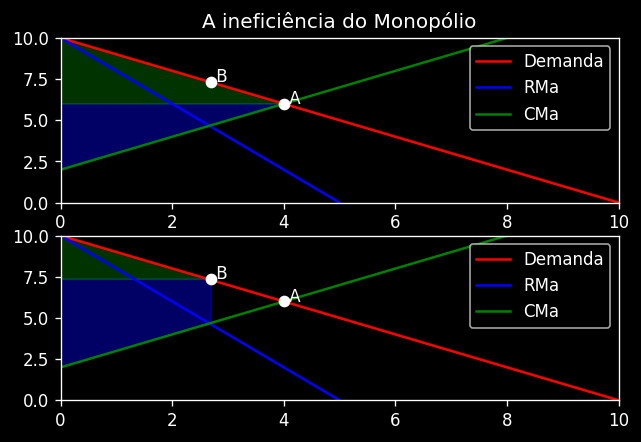
\includegraphics[scale=0.6]{cap25_4-inef_monopolio.png}
	\end{center}
\end{frame}

\begin{frame}
	\frametitle{A Ineficiência do Monopólio}
	
	O gráfico da parte de cima é o equilíbrio no mercado de competição e o de baixo é o nosso equilíbrio com monopólio.
	\\~\\
	Perceba como há um incremento no excedente do produtor (medido pela área azul) e uma redução do excedente do consumidor (área verde).
	\\~\\
	Para investigarmos se há uma ineficiência no sentido de Pareto no ponto $B$, façamos a seguinte pergunta: 
	\begin{block}{Para discussão em aula}
		É possível adicionar uma unidade de produto no mercado de modo que o custo marginal pela produção desse bem seja inferior ao preço do mesmo?
	\end{block}	
\end{frame}

\begin{frame}
	\frametitle{A Ineficiência do Monopólio}
	
	No nível $B$, a curva de preço (medida pela demanda inversa) ainda é superior à curva de custo marginal (aquela reta verde).
	\\~\\
	Desse modo, se o monopolista produzisse mais uma unidade, ele receberia mais do que o custo marginal dessa unidade e os consumidores cujo preço de reserva é igual ao novo nível de preço passariam a consumir o produto.
	\\~\\
	Como o produtor teria um lucro positivo (pois o custo marginal é inferior ao preço) e os consumidores teriam um aumento de excedente, achamos uma melhoria de Pareto.
	\\~\\
	Com isso, podemos ver que o equilíbrio com monopólio é ineficiente no sentido de Pareto.
\end{frame}

%%%%%%%%%%%%%%%%%%%%%%%%%%%%%%%%%%%%%%%%%%%

\begin{frame}
	\frametitle{O Ônus do Monopólio}
	
	Agora que já vimos que o monopólio é ineficiente, podemos querer mensurar o tamanho dessa ineficiência.
	\\~\\
	Uma maneira possível de medir essa ineficiência é observando os excedentes nos cenários competitivo e de monopólio. Observe a figura abaixo:
	
	\begin{center}
		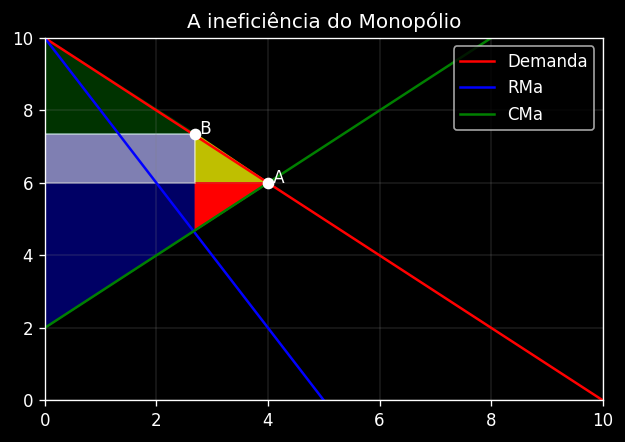
\includegraphics[scale=0.5]{cap25_5-onus_monopolio.png}
		\end{center}
\end{frame}

\begin{frame}
	\frametitle{O Ônus do Monopólio}
	
	A área amarela é a medida da redução do excedente do consumidor.
	\\~\\
	Em vermelho temos a redução do excedente do produtor.
	\\~\\
	Em branco temos o quanto o monopolista consegue "capturar"\ do excedente dos consumidores ao adotar o nível de produção que maximiza o seu lucro.
	\\~\\
	O \textbf{ônus resultante do monopólio} é precisamente a soma das áreas amarela e vermelha.
\end{frame}

%%%%%%%%%%%%%%%%%%%%%%%%%%%%%%%%%%%%%%%%%%%

\begin{frame}
	\frametitle{O Monopólio Natural}

	Já aprendemos o modelo de decisão do monopolista e também já vimos a ineficiência que esse modelo acarreta para os mercados.
	\\~\\
	Ao percebemos que o monopólio produz aquém da quantidade ótima, poderíamos nos sentir tentados a propor regulações que obrigassem o monopolista a aumentar o seu nível de produção até o nível da competição perfeita.
	\\~\\
	Contudo, esse problema é mais complexo do que parece, porque essa proposta de solução não leva em consideração a estrutura de custos.
	\\~\\
	A próxima imagem é um exemplo do que acontece quando alteramos apenas o custo fixo em 3 diferentes cenários.
\end{frame}

\begin{frame}
	\frametitle{O Monopólio Natural}
	\begin{center}
		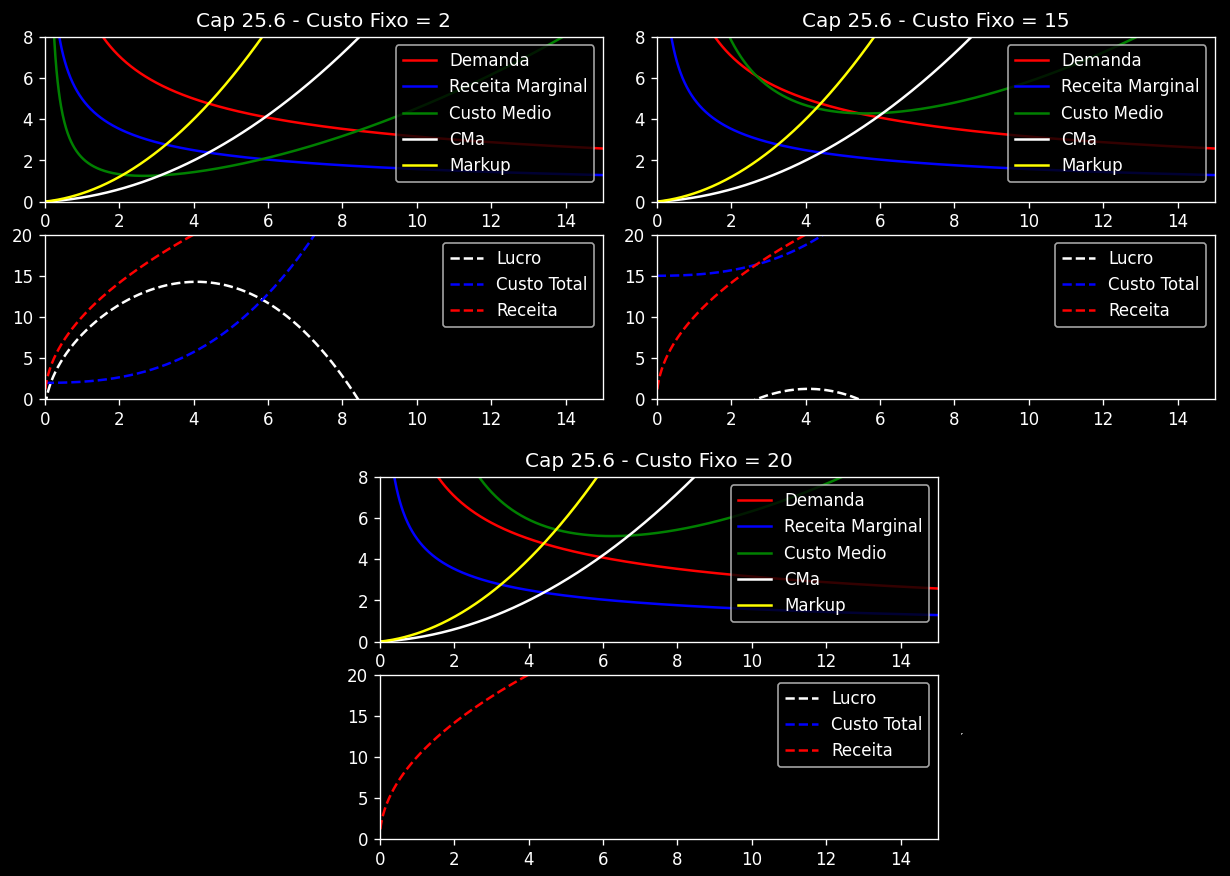
\includegraphics[scale=0.3]{cap25_6-monopolio_natural.png}
		\end{center}
\end{frame}

\begin{frame}
	\frametitle{O Monopólio Natural}

	Chamamos de \textbf{monopólio natural} a situação onde temos uma estrutura de custo fixos muito alta e custos marginais baixos.
	\\~\\
	Agora podemos ver que se obrigarmos o monopolista a produzir o nível da competição perfeita, pode acontecer do projeto não ser sustentável, pois a curva de custo médio está acima da curva de demanda.
	\\~\\
	Não existe solução simples para essa questão. Na maioria das situações os monopólios naturais são regulamentados ou operados diretamente pelos governos.
	\\~\\
	Cada opção de solução acaba acarretando benefícios e malefícios consigo. Em ambos os casos, os problemas são geralmente oriundos devido a informação assimétrica entre a empresa e os seus controladores.
\end{frame}

%%%%%%%%%%%%%%%%%%%%%%%%%%%%%%%%%%%%%%%%%%%

\begin{frame}
	\frametitle{O que Causa os Monopólios?}

	Agora nos resta uma última investigação: Qual a causa dos monopólios?
	\\~\\
	Uma variável que podemos creditar como importante é a \textbf{escala mínima de eficiêntia (EME)}. Ela nada mais é do que o ponto de mínimo da nossa curva de custo médio.
	\\~\\
	O formato da curva de custo médio (e consequentemente a EME) é definido exclusivamente pela tecnologia.
	\\~\\
	Quando temos uma escala mínima de eficiência muito elevada, uma empresa precisa produzir uma quantidade muito grande dos bens vendidos no mercado para se manter.
\end{frame}

\begin{frame}
	\frametitle{O que Causa os Monopólios?}
	Quando temos uma EME pequena, qualquer empresa pequena pode começar a operar no mercado. Isso aumenta o número de competidores.
	\\~\\
	O que acaba por reduzir o peso de cada empresa individualmente. O que acaba por gerar um ambiente de competição.
	\\~\\
	Observe que o fator importante é a relação entre a EME e o tamanho do mercado. Se a EME é de 10.000 unidades, mas o mercado é o país todo, essa é uma EME relativamente baixa. Se o tamanho do mercado fosse um único shopping center, aí seria considerar consideravelmente alta.
\end{frame}

\begin{frame}
	\frametitle{O que Causa os Monopólios?}
	Além da EME, outra maneira de se criar um monopólio é por meio da coordenação dos agentes ofertantes em uma \textbf{colusão}.
	\\~\\
	Quando um conjunto de empresa se une para definir em conjunto a produção, elas agem como um \textbf{cartel}.
	\\~\\
	Esse cartel acaba atuando como se fosse um ofertante só (e consequentemente, age com o poder de mercado advindo dessa coordenação).
\end{frame}

\begin{frame}
	\frametitle{O que Causa os Monopólios?}
	Um terceiro e último motivo para o nascimento de um monopólio é o bom e velho "cheguei primeiro".
	\\~\\
	Se uma empresa, por algum acidente histórico, é a primeira a se estabelecer no mercado. É natural que ela se valha da falta de competidores e consiga um crescimento em escala.
	\\~\\
	Quando novos ofertantes entram no mercado, o monopolista consegue usar seu arsenal de escala e reduzir artificialmente o preço até o ponto onde ninguém além dele pode se manter.
\end{frame}

\end{document}

